	\documentclass{llncs}

\usepackage{url}
\usepackage[pdftex]{graphicx}
\usepackage{listings}
\usepackage{verbatim}
\usepackage[lined,linesnumbered,algochapter]{algorithm2e}
\usepackage{tikz}
\usetikzlibrary{arrows,automata}
\usepackage{xspace}
\usepackage {pdfsync}
\usepackage{amsmath}

\usepackage{ngerman}
\usepackage[ngerman, english]{babel}
\usepackage{bibgerm,cite}       % Deutsche Bezeichnungen, Automatisches Zusammenfassen von Literaturstellen
\usepackage[ngerman]{varioref}  % Querverweise

\setcounter{secnumdepth}{2}
\setcounter{tocdepth}{3}

% define custom macros for specific formats or names
\newcommand{\uml}[1]{\texttt{#1}}
\newcommand{\cd}{\textsf{Class Diagram}}

\begin{document}
\pagestyle{plain}
\pagenumbering{roman}

\title{Towards Systematic Mutations for and with ATL Model Transformations\footnote{This work has been created in the context of the course ``188.952 Advanced Model Engineering (VU 2,0)'' in SS15.}}


%&&&&&&&&&&&&&&&&&&&&&&&&&&&&&&&&&&&&&&&&&&&&&&&&&&&&&&&&&&&&&&&&&&&&&&&&
% Name and address of the author
%&&&&&&&&&&&&&&&&&&&&&&&&&&&&&&&&&&&&&&&&&&&&&&&&&&&&&&&&&&&&&&&&&&&&&&&&
\author{Patrick Sommer\inst{1} and Carola Gabriel\inst{2} and Martin Keiblinger\inst{3}}

\institute{Mautner Markhof-Gasse 58/4/31, 1110 Wien \\ \email{e0925011@student.tuwien.ac.at} \\ MatrNr.: 0925011
\and
Mustergasse 54/4/3, 1030 Wien \\ \email{matthias@tuwien.ac.at} \\ MatrNr.: 0426553
\and
Mustergasse 54/4/3, 1030 Wien \\ \email{matthias@tuwien.ac.at} \\ MatrNr.: 0426553
}

\maketitle

\begin{abstract}

This abstract summarizes the content of this paper in about 70 to 150 words. \dots
\end{abstract}

%&&&&&&&&&&&&&&&&&&&&&&&&&&&&&&&&&&&&&&&&&&&&&&&&&&&&&&&&&&&&&&&&&&&&&&&&
% Table of contents
% Activate or deactivate this according to the guideline instructor
%&&&&&&&&&&&&&&&&&&&&&&&&&&&&&&&&&&&&&&&&&&&&&&&&&&&&&&&&&&&&&&&&&&&&&&&&
\tableofcontents
%\thispagestyle{plain}
\newpage

\pagenumbering{arabic}

\section{Introduction}

The broader goal of this work is to create an introduction to a specific field of software testing. Software testing is a process, or a series processes engineered to check if a program does what it is designed to do and that id does not do anything unintended.\cite{Myers:2004} Model based testing (MBT) is a variant of testing. Test cases are not written by the programmer directly. The programmer creates a model of the requirements and in a second step the test cases are generated on base of the model.\cite{Utting:2012}

Mutation testing is a fault-based testing technique. It applys changes to the input and creates a mutant. A mutant represents a faulty program. In the best case these changes, which are applied by the mutator, represent mistakes a programmer would make.\cite{mutationssurvey:yue}

The basic idea is of mutation testing is not to test the resulting software itself but the test cases. Good test cases should be able to identify mutants. Identifying means recognizing differing results of the original system under test (SUT) or mutants.\cite{MatMottu2006}

The process of mutation testing consists of these components:
\begin{itemize}
	\item \textit{Test data} as input for the original programm P and its mutants.
	\item The original program \textit{P}
	\item The \textit{mutants} of P.
	\item An \textit{oracle} which is able to decides if results differ and which is therefore able to identify mutants.
\end{itemize}

\begin{figure}
	\centering
	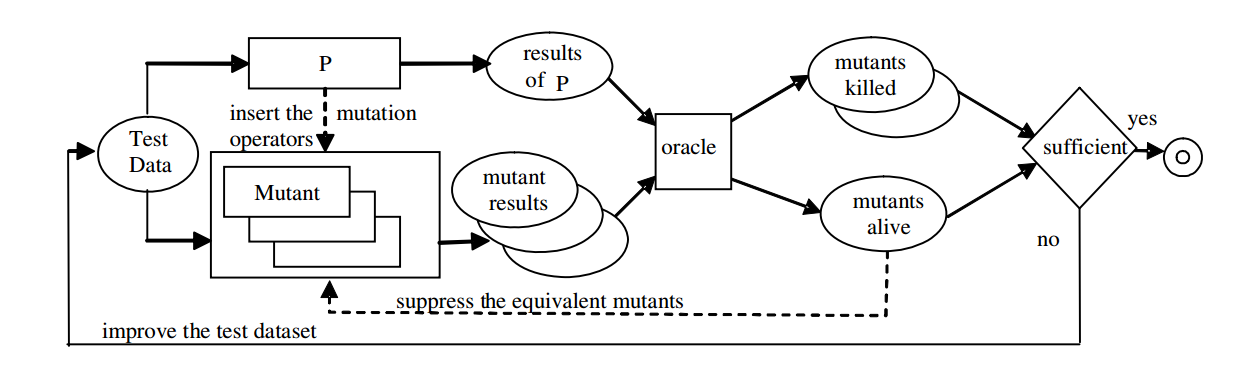
\includegraphics[width=0.7\textwidth]{figures/Mutation_Process}
	\caption{The mutation testing workflow contains a feedback loop.\cite{MatMottu2006}}
	\label{fig:Mutation_Process}
\end{figure}

The goal of the process\ref{fig:Mutation_Process} is to \textit{kill} or identify faulty versions of P. If a mutant outputs the same data as the P for the same input data it's called \textit{equivalent}. In this case this mutant has to removed from the set of mutants under test.

The last step is to assess how good the tests are and check if they should be improved. Assume \textit{KM} as the set of the killed mutants, \textit{M} is the set of all mutants and \textit{EM} is the set of all identified, equivalent mutants. Then the mutation score \textit{MS} is calculated like this:\cite{mutationssurvey:yue}

\begin{equation}
	MS = \frac{\left|KM\right|}{\left|M\right| - \left|EM\right|}
	\label{eq:ms}
\end{equation}

If this value is to small the tests have to be improved. 

The success of this method depends on the set of mutants used in the process. Manual creation of mutants is a tedious and time consuming task. Therefore a quick, reliable and efficent creation of mutants is proposed in \cite{troya:2015}.

Troya et. al. build upon ATL and higher order transformations (HOT) to create transformations to automatically generate mutants. 

This report show what additional transformation have been developed and what their goal is. The scope of this work is only on the mutation generation in the whole process.

\begin{figure}
	\centering
	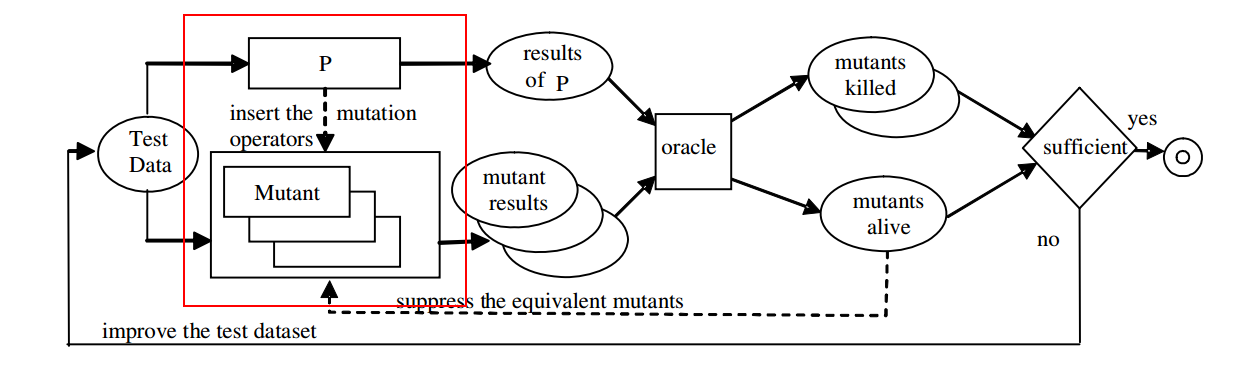
\includegraphics[width=0.7\textwidth]{figures/Marked_Mutation_Process}
	\caption{The mutation testing workflow contains a feedback loop.\cite{MatMottu2006}}
	\label{fig:Marked_Mutation_Process}
\end{figure}

\section{General}

Model transformations play an important role in the Model Driven Engineering
(MDE) approach. Developing model transformation definitions is expected to
become a common task in model driven software development. \cite{atl:frederic}
In this part of the paper we want to explain the basics of the requirements we needed for Mutations for and with ATL Model Transformations.

\subsection{Model transformation in MDE}
Model transformation is an important technique in software development, espacially in Model-Driven Software Development (MDSD) and Model-Driven Software Development (MDA). There exists different types of model transformations like Model-To-Model Transformation and Model-To-Text Transformation.  

\subsection{ATL}
ATL is a model transformation language containing a mixture of declarative and
imperative constructs. ATL is applied in the context of the
transformation pattern shown in \label{fig:overview_atl}. In this pattern a source model Ma is transformed into a target model Mb according to a transformation definition mma2mmb.atl written in the ATL language. The transformation definition is a model conforming to the ATL metamodel. All metamodels conform to the MOF.
ATL is a hybrid transformation language. It contains a mixture of declarative
and imperative constructs. We encourage a declarative style of specifying transformations. The declarative style of transformation specification has a number of advantages. It is usually based on specifying relations between source and target patterns and thus tends to be closer to the way the developers intuitively perceive a transformation. This style stresses on encoding these relations and hides the details related to selection of source elements, rule triggering and ordering, dealing with traceability, etc. Therefore, it can hide complex transformation algorithms behind a simple syntax.\cite{atl:frederic}

\begin{figure}
	\centering
	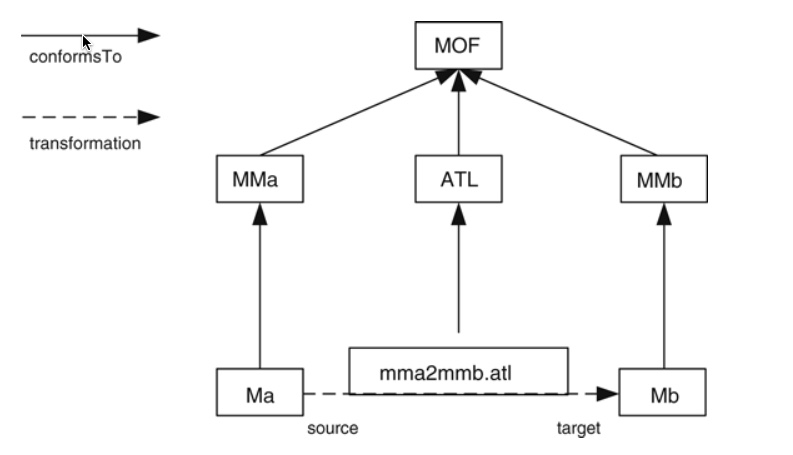
\includegraphics[width=0.7\textwidth,natwidth=610,natheight=642]{figures/Overview_ATL.jpg}
	\caption{Overview of the ATL transformational approach}
	\label{fig:overview_atl}
\end{figure}~\cite{atl:frederic}

\begin{figure}
	\centering
	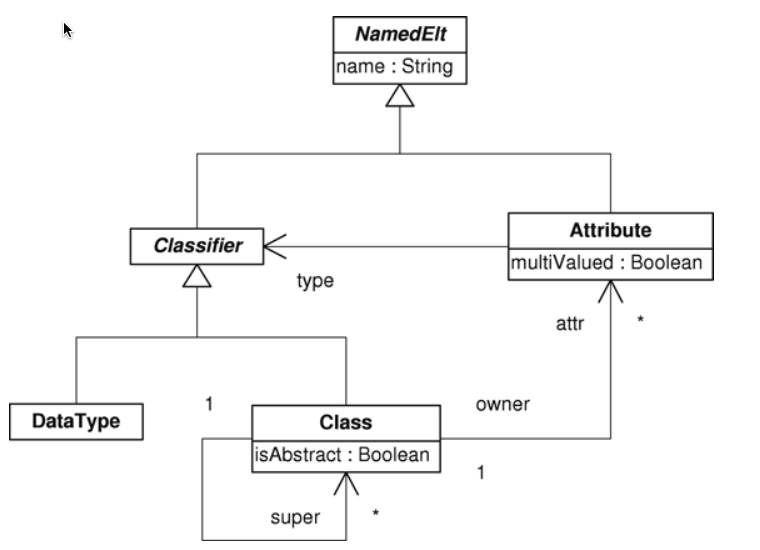
\includegraphics[width=0.7\textwidth,natwidth=610,natheight=642]{figures/Class_metamodel.jpg}
	\caption{Class metamodel}
	\label{fig:class_metamodel_atl}
\end{figure}~\cite{atl:frederic}

\begin{figure}
	\centering
	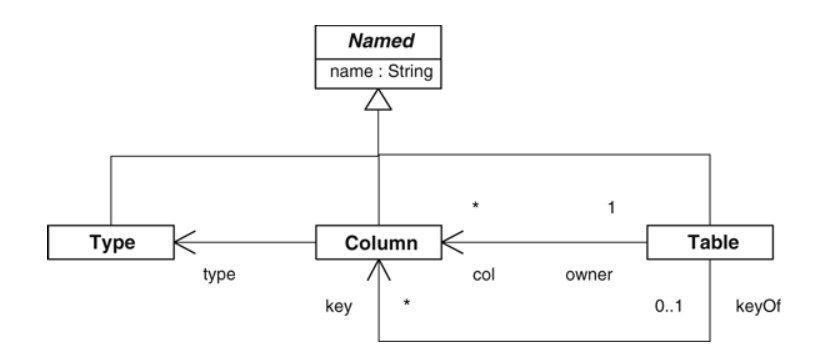
\includegraphics[width=0.7\textwidth,natwidth=610,natheight=642]{figures/Relational_metamodel.jpg}
	\caption{Relational metamodel}
	\label{fig:relational_metamodel_atl}
\end{figure}~\cite{atl:frederic}

In the following you can see a short example of a ATL transformation:
\begin{verbatim}
//Start Program
module Entities2Forms;
create OUT : Forms from IN : Forms;

rule EntityModel2FormModel {
	from
		em : Forms!EntityModel
	to 
		fm : Forms!FormModel (
		)
}
//End Program
\end{verbatim}

This ATL file shows a tranformation Entities2Form. The source model is the 'IN'
model and the target model is 'OUT'. The rule mapped the elements EntityModel to
FormModel. 


\subsection{High Order Transformations}

Higher order transformations is a model transformation such that its input and/or output models are themselves transformation models.\cite{Tisi:2009}

Therefore a transformation model is:

\begin{itemize}
	\item The input of a HOT
	\item The output of a HOT
	\item Or it is both
\end{itemize}

Tisi et. al identified four transformation patterns for HOTs:

\begin{itemize}
	\item \textbf{Transformation Synthesis} These HOTs generate transformations. If any input is used it's not a transformation.
	\item \textbf{Transformation Analysis} take transformations as input and generate data of different kinds as output. The output is never a transformation.
	\item \textbf{Transformation (De)composition} is the integration of multiple transformations of the input and/or integration of transformations as output.
	\item \textbf{Transformation Modification} is defined by modifing an input transformation and generating an output transformation.
\end{itemize}

The focus of this work is on \textit{Transformation Modifications} (short TM). 

\subsection{Mutations in Model Transformations}

\begin{figure}[tb]
	\centering
	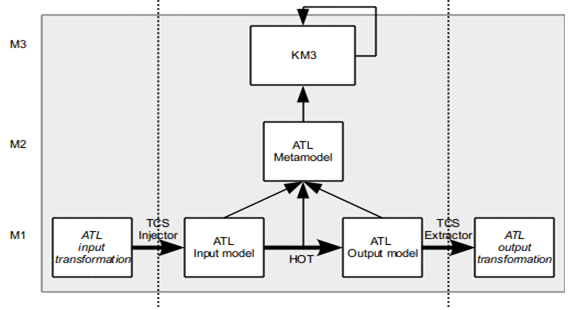
\includegraphics[width=0.7\textwidth,natwidth=610,natheight=642]{figures/HOT.png}
	\caption{Sample schema of a HOT for transformation modification in ATL}
	\label{fig:samplefigure_pdf}
\end{figure}~\cite{misc:ModelingLanguages}

\section{Implementation}

\subsection{Transformations}

\subsubsection{Binding}

\textbf{Addition}

\textbf\textit{{Implementation}}

\textbf\textit{{Discussion}}

\textbf{Deletion}

\textbf\textit{{Implementation}}

\textbf\textit{{Discussion}}

\textbf{Change}

\textbf\textit{{Implementation}}

\textbf\textit{{Discussion}}

\subsubsection{Out Pattern Element}

\textbf{Addition}

\textbf\textit{{Implementation}}

\textbf\textit{{Discussion}}

\textbf{Class change}

\textbf\textit{{Implementation}}

\textbf\textit{{Discussion}}

\subsubsection{In Pattern Element}

\textbf{Deletion}

\textbf\textit{{Implementation}}

\textbf\textit{{Discussion}}

\textbf{Class change}

\textbf\textit{{Implementation}}

\textbf{Discussion}

Explain what we did and why.

\subsection{Related transformation}

Explain what other transformations would make sense.

\section{Conclusion}

\section{Bibliographic Issues}

\subsection{Literature Search}

Information on online libraries and literature search, e.g., interesting magazines, journals, conferences, and organizations may be found at \url{http://www.big.tuwien.ac.at/teaching/info.html}.

\subsection{BibTeX}

BibTeX should be used for referencing.

The LaTeX source document of this pdf document provides you with different samples for references to journals~\cite{jour:B2BServices}, conference papers~\cite{proc:TheWebMLApproach}, books~\cite{book:umlatwork}, book chapters~\cite{incoll:ErhardKonrad1992}, electronic standards~\cite{man:BPEL}, dissertations~\cite{phdthesis:manuelWimmer}, masters' theses~\cite{mast:AUMLProfile}, and web sites~\cite{misc:BIGWebsite}. The respective BibTeX entries may be found in the file \texttt{references.bib}. For administration of the BibTeX references we recommend \url{http://www.citeulike.org} or JabRef for offline administration, respectively.

\bibliographystyle{acm}
\bibliography{references}

\end{document}
